\documentclass[12pt]{article}
\usepackage[english]{babel}
\usepackage{natbib}
\usepackage{url}
\usepackage[utf8x]{inputenc}
\usepackage{amsmath}
\usepackage{graphicx}
\graphicspath{{images/}}
\usepackage{parskip}
\usepackage{fancyhdr}
\usepackage{vmargin}
\setmarginsrb{3 cm}{2.5 cm}{3 cm}{2.5 cm}{1 cm}{1.5 cm}{1 cm}{1.5 cm}

\title{Communication Engineering}								% Title
%\author{13103057}								% Author
\date{28 Oct 2018}											% Date

\makeatletter
\let\thetitle\@title
\let\theauthor\@author
\let\thedate\@date
\makeatother

\pagestyle{fancy}
\fancyhf{}
\rhead{\theauthor}
\lhead{\thetitle}
\cfoot{\thepage}

\begin{document}

%%%%%%%%%%%%%%%%%%%%%%%%%%%%%%%%%%%%%%%%%%%%%%%%%%%%%%%%%%%%%%%%%%%%%%%%%%%%%%%%%%%%%%%%%

\begin{titlepage}
	\centering
    \vspace*{0.5 cm}
    
\includegraphics[scale = 0.75]{iitd.jpg}\\[1.0 cm]	% University Logo
    \textsc{\LARGE Indian Institute of Technology\newline\newline Delhi}\\[2.0 cm]	% University Name
	\textsc{\Large ELL-311}\\[0.5 cm]				% Course Code
	\rule{\linewidth}{0.2 mm} \\[0.4 cm]
	{ \huge \bfseries \thetitle}\\
	\rule{\linewidth}{0.2 mm} \\[1.5 cm]
	
	\begin{minipage}{0.4\textwidth}
		\begin{flushleft} \large
			\emph{Submitted To:}\\
			Prof. Saif K. Mohhamed\\
			\end{flushleft}
			\end{minipage}~
			\begin{minipage}{0.4\textwidth}
            
			\begin{flushright} \large
			\emph{Submitted By :} \\
			Gantavya Bhatt\\
			(2016EE10694)\\
			Snigdha Dalvi\\
			(2016EE30529)\\
			Kashish Jain\\
			(2016EE10434)\\
		\end{flushright}
        
	\end{minipage}\\[2 cm]
	
	
    
    
    
    
	
\end{titlepage}

\section*{Contents}
\subsubsection*{Problem Statement}
\subsubsection*{Definitions and Mathematical Analysis}
\subsubsection*{Mathematical Derivation}
\subsubsection*{Delay Decoding}
\subsubsection*{Simulations}
\subsubsection*{Multiple Object Detection}
\subsubsection*{Effect of Noise on Spectrum}
\subsubsection*{Results and Discussions}
\pagebreak
\section{Problem Statement}
\begin{flushleft}
\begin{itemize}
    \item Give the mathematical expressions for the transmitted and the received signal (reflected from an object) at the radar, and show how  they can be used together to get an estimate of the distance of the reflecting object from the Radar. 
    \item Will the signal processing performed by you to detect the distance of the reflecting object work if there are two different reflecting objects? (Support your answer with theoretical analysis and simulations).
    \item In part-I, is there any practical limitation on the maximum distance of the reflecting object that can be measured accurately? Do you think noise at the radar receiver, and the energy of the signal transmitted from the radar could impact the practical range of the radar? (In parts Q1, and Q2 no noise has been assumed at the Radar receiver, however in Q3 let us consider noise at the Radar receiver and analyze its impact through analysis/Matlab simulation).
\end{itemize}
\end{flushleft}
\section{Definitions and Mathematical Analysis}
\begin{flushleft}
The Transmitted signal is defined as
\[y(t) = cos(2\pi f_ct + 2\pi k_f \int_{0}^{t} m(x) dx)\]
The m(t) is the message signal and through that we are going to detect the postion of any flying object. In this model that m(t) that we are using is a triangle signal. The parameters of the message signal are its amplitude defined as $\Delta$f and the frequency being $f_0$. It is shown as follows :-\\
\begin{center}
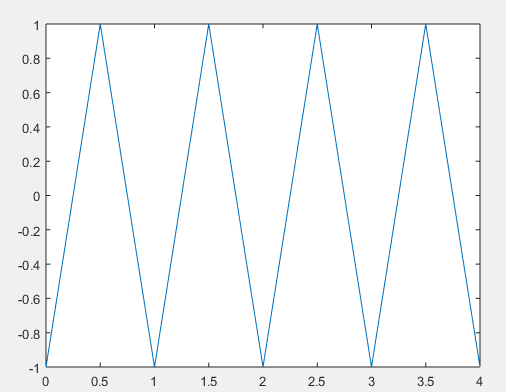
\includegraphics[scale = 0.6]{message.PNG}\\[1.0 cm]
\end{center}
\end{flushleft}
\begin{flushleft}
Above is the message signal that has a peak to peak amplitude of 2V. This would be varied for different values of the delay that we will recieve.\\
The signal that we will receive would be a delayed version of the signal y(t). \\
\textit{\textbf{Note that the signal so received would also contain a phase difference of $\pi$ but in the process where we will be mixing it with the transmitted signal and further passing it through a Low pass filter, the useful information will not be affected by the sign of the signal(since $\pi$ difference can only change sign). }}'
\\
Received signal would be y(t-$\tau$). Mathematically it could be written as :- \[y(t-\tau)  = cos(2\pi f_c(t-\tau) + 2\pi k_f \int_{0}^{t- \tau} m(x) dx + \pi ) \]
\textit{From Now onwards, we will not write the phase difference $\pi$ and won't consider the sign introduced by it. \\}

After passing it through a mixer, that is the multiplication operator with the transmitted signal and further with a LPF, we will recieve the following signal call it as r(t)
\[r(t) = cos(2\pi f_c\tau+2\pi k_f \int_{t- \tau}^{t} m(x) dx )\]
The frequency is defined as :-
\[f = \frac{1}{2\pi}\frac{d\phi}{dt}\]
where $\phi$ is the instantaneous phase of the system. In this system, our instantaneous frequency-f would be :-
\[f = k_f(m(t) - m(t-\tau))\]
For a saw tooth wave, the instantaneous frequency will look like :- \\
\begin{center}
    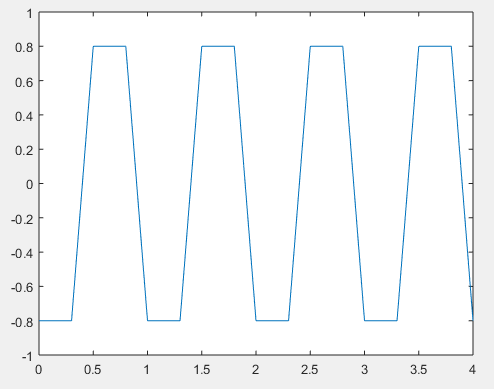
\includegraphics[scale = 0.55]{diff.PNG}\\[1.0 cm]
    %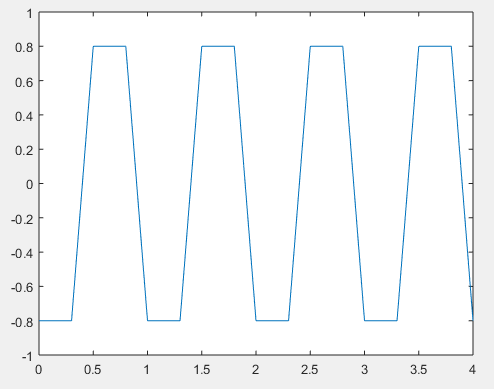
\includegraphics[width=1\textwidth]{diff.PNG}
    \caption{\label{fig:diff.PNG}{For some $\tau$ the freq of LPF output}}
\end{center}
As we keep on increasing the $\tau$ and reach the half of time period as the delay, we will have the following time series for frequency :- \\
\begin{center}
     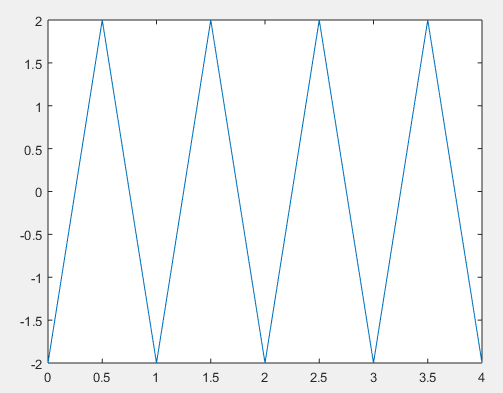
\includegraphics[scale = 0.55]{diff4.PNG}\\[1.0 cm]
    \caption{\label{fig:diff.PNG}{For $\tau =\frac{1}{2f_0} $ the freq of LPF output}}
\end{center}
If we reduce the value of delay to very low values as compared to $\frac{1}{2f_0}$ we will get the following time series  :- \\
\begin{center}
     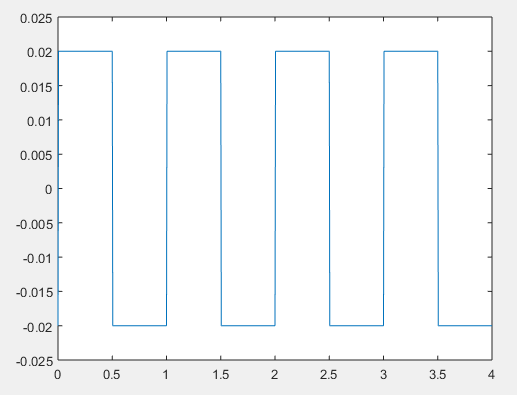
\includegraphics[scale = 0.55]{diff0.PNG}\\[1.0 cm]
    \caption{\label{fig:diff.PNG}{For some $\tau << \frac{1}{2f_0}$ the freq of LPF output}}
\end{center}
It can be seen that as we decrease the value of $\tau$ the frequency of the system turns more and more to a square wave and as it reaches the half of time period, it becomes a triangular wave. Also at low $\tau$, the peak frequency is decreasing as comapred to higher $\tau$. In the next section we will mathematically derive the expressions for the apmlitude and time period of the frequency function.
\end{flushleft}
\section{Mathematical Derivation}
\begin{flushleft}
In one time period, we can define our message signal m(t) as - \\
\[ m(t)=   \left\{
\begin{array}{ll}
      -4\Delta ff_o t+ \Delta f  & 0 \leq t\leq \frac{1}{2f_o} \\
       4\Delta ff_o t-3\Delta f  & \frac{1}{2f_o} \leq t \leq \frac{1}{f_o}
\end{array} 
\right. \]
The signal m(t-$\tau$) will be its shifted version and:- \\
\[ m(t-\tau)=   \left\{
\begin{array}{ll}
      -4\Delta ff_o (t-\tau)+ \Delta f  & \tau \leq t\leq \frac{1}{2f_o}+\tau \\
       4\Delta ff_o (t-\tau)-3\Delta f  & \frac{1}{2f_o}+ \tau \leq t \leq \frac{1}{f_o}+ \tau
\end{array} 
\right. \]
So we can say that in a period, the frequency which is the difference of the two would be :-
\[ m(t) - m(t-\tau)=   \left\{
\begin{array}{ll}
      -8\Delta ff_o t+ 4\Delta ff_o\tau &  0 \leq t\leq \tau \\
      -4\Delta ff_o\tau                 & \tau \leq t \leq \frac{1}{2f_o}\\
      8\Delta ff_o t -4\Delta -4\Delta ff_o \tau & \frac{1}{2f_o} \leq t \leq \frac{1}{2f_o} + \tau \\
      4\Delta ff_o\tau                                   & \frac{1}{2f_o} +\tau \leq t \leq \frac{1}{f_o}
\end{array} 
\right. \]
\subsection*{Observation}
\begin{flushleft}
Thus from the above mathematical equation, its clear that the amplitude of the frequency of the LPF output is $4\Delta ff_o\tau k_f$. Also the time for which the mod of frequency is $4\Delta ff_o\tau k_f$ is $\frac{1}{2f_o} - \tau$ and similarly for the -ve part. \\
\textit{\textbf{*Note that the -ve frequency is just the phasor rotating in the negative direction. The power contained in the frequency is same as that of in the +ve part.
}}\end{flushleft}
\end{flushleft} 
\subsection*{Analysis of delay}
\begin{flushleft}
The delay in the received wave is of $\tau$. How large can be this delay for a good waveform? \textit{\textbf{From the above mathematical derivation, its clear that for the flat region of the frequency to exist, we should have the condition that \textbf{$\tau \leq \frac{1}{2f_o}$}.}} However, when the delay $\tau \geq \frac{1}{2f_o}$ we the frequency equation will remain similar to that we had derived in the earlier part just we need to replace the $\tau$ with $\frac{1}{f_o}-\tau$ because of the symmetry of the problem.\\
Thus, the amplitudes remain the same, but the time for flat frequency changes from  $\frac{1}{2f_o} - \tau$ to  $\tau-\frac{1}{2f_o}$ and the slant regions also changes accordingly.\\

\subsection*{Average Beats}
\begin{flushleft}
From the graph and also from the equation of frequency, we will determine the average frequency(or in more lamer language, the number of zero crossings in a second). The total number of beats in a time period will be 2 times the area of the trapezium so formed by the equation of the beat frequency. \\
Let N be the total number of beats in a time period. Then N would be equal to :- \\
\[N = 2(4\Delta ff_o\tau(\frac{1}{2f_o}-\tau) + 2\Delta ff_o\tau^2)\]
\[N = 4\Delta f\tau(1-f_o\tau)\]
So average N per second is - 
\[<f_{beat}> =4\Delta ff_o\tau(1-f_o\tau) \]
It can be verified by inspection that by shifting the $\tau$ by any amount shouldn't change the beat frequency, this could also be seen by the quadratic equations that we had obtained.
\textbf{\textit{Note that the solutions of the quadratic equation can lead us to the possible values of the delay $\tau$. Since its a quadratic equation, it will have 2 roots. Also Note that if $\tau$ is the solution of the equation, then $\frac{1}{f_o}- \tau$ is also a solution of the equation.}}
\end{flushleft}
\end{flushleft}
\section{Delay Decoding}
\begin{flushleft}
The main goal of our exercise is to determine the distance of the target object using the FM transmission. The distance and delay are linearly related by \textbf{$\tau = \frac{2d}{c}$ }where c is speed of light in the medium (free space in our case). We have 2 methods to determine the delay from the mixer and LPF output. 
\begin{item}
    \item 1)Using FFT to the filtered output and then determining the frequency and relating it to delay.
    \item 2)Counting the number of zero crossings and then equating it with the quadratic equation to determine the values of $\tau$.
\end{item}
\subsection*{About Simulation}
To simulate the similar environment by our simplified model, we will choose some values of $\tau$ to get the mixed LPF output. Further from that, we will evaluate the $\tau$ from our above mentioned mathematical analysis and techniques. In the end we will find the error between our calculated value of delay with the actual value of delay provided at the starting of our simulation. In the end we will discuss the theoretical error and noise analysis.
\subsection*{Simulation Limitations}
\begin{itemize}
    \item The simulation is done on MATLAB and on a system i3, 4th generation. Because of allowed memory to the program by the Operating system as well as the less parallel computation, \textbf{we wont be able to have high sampling frequency and won't be able to simulate the very small values of delay }\textit{ $\tau$} or very high frequencies.\textit{\textbf{ However, we will see the effect of changing delay $\tau$ and other parameters on our simulations.\\}}
    \item Since the sampling frequency cannot simply be very high because of simulation overhead, we cannot find the exact number of zero crossings and so can't simulate the second method with less error. \textbf{\textit{However, we will give some possible method to implement that at simulation platform.}}
\end{itemize}
\end{flushleft}
\section{Simulations}
In this section we will show how we did the simulation and their results. 
\subsection*{Beat frequency Method: Time domain analysis}
\begin{flushleft}
As discussed above, this method is computationally expensive and will cause much error in the output because of overhead of sampling frequency. However to implement this method we will have to count the number of sign changes of the r(t) which requires that the sampling frequency to be greater than the maximum frequency. 
After counting the number of zeroes in 1 second, we will equate this to the quadratic of
\[count = 4\Delta ff_o\tau(1-f_o\tau)\]
from this quadratic equation, we will get the value of $\tau$
\subsubsection*{Drawbacks and Limitations}
In this method, we don't know the values of the function r(t). Also to simulate this we will require the sampling frequency greater than the maximum frequency(derived from the Carson's Bandwidth rule). \textbf{\textit{Since this method involve the calculation of zeros, its highly probable that noise will cause tremendous error. Hence if we have to employ this, then we need to choose the region boundaries that decide whether to count something as positive or negative in the presence of noise. Thus this would be a stochastic variable.}} Hence for the sake of simulation we won't simulate this. Thus we will show results from the frequency domain analysis.\\

\end{flushleft}
\subsection*{Fast Fourier Transform: Frequency Domain Analysis}
In this analysis, we will use the Fast Fourier transform to get the power spectral density of the signal. As we have seen that the frequency is mostly comprising of the flat region one, so we will have maxima of power spectral density at the frequency corresponding to the flat region.\\
\subsubsection*{Frequency Bins to frequency}
The Fourier transform will be in units of bins. We can convert the frequency output in bins to that of in Hertz by the simple conversion as show here - 
\[f_{hertz} = \frac{x}{Tmax}\]
Where x is the freq in bins and Tmax is the maximum time interval to which we are simulating in the time domain
\subsubsection*{Constraints}
During the simulations, we have made the following constraints:-
\begin{itemize}
    \item $\tau \leq \frac{1}{2f_o}$. We had justified this constraint in the above mathematical discussions. \textbf{\textit{This will set the practical limit on the radar range for fixed value of frequencies}}
    % \item Actual flat freq is $k_f 4\Delta ff_o\tau$. To represent this on the scale we must have  $k_f 4\Delta ff_o\tau \leq \frac{1}{2t_s}$
\end{itemize}
\begin{flushleft}
As of simulation results we will show the effect of changing parameters and our output as compared to real answer.
\end{flushleft}
\subsubsection*{Observations for single Object detection}
\begin{flushleft}
Here we present the results by changing the distance(i.e. changing the delay) $\tau$ and see its effect on the Spectral density distribution. Also we will change the parameters of the system (modulation index, signal amplitude and frequency) to see what is the their effect while keeping the delay constant.
\subsubsection*{Effect of Changing delay}
The central frequency, $f_o$ are scaled down in corresponding ratio to make sure the computation can be done. Sampling time= 0.001s, Tmax = 1s, $f_o = 5Hz$,  fc = 100Hz, kf=10 $\Delta$ f= 10. \\
Following figures are at the delay values 0.002, 0.015, 0.045, 0.065 and 0.095 sec. respectively.
\begin{center}
    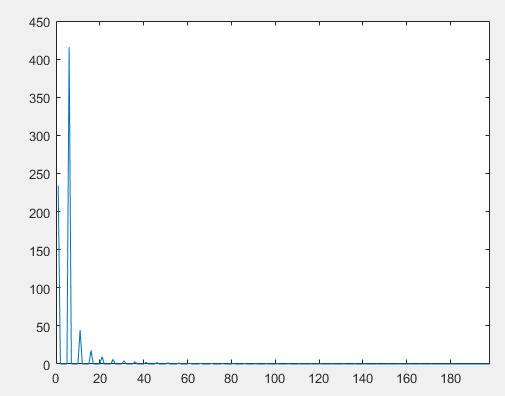
\includegraphics[scale = 0.75]{_002.PNG}\\[1.0 cm]
    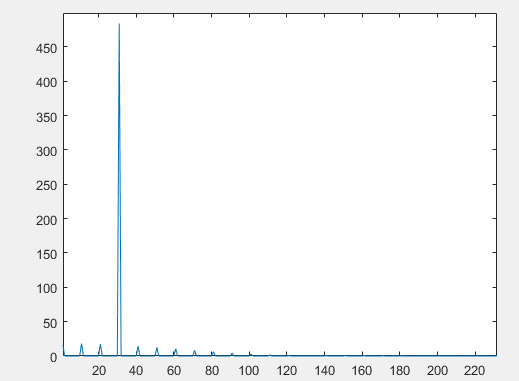
\includegraphics[scale = 0.75]{_015.PNG}\\[1.0 cm]
    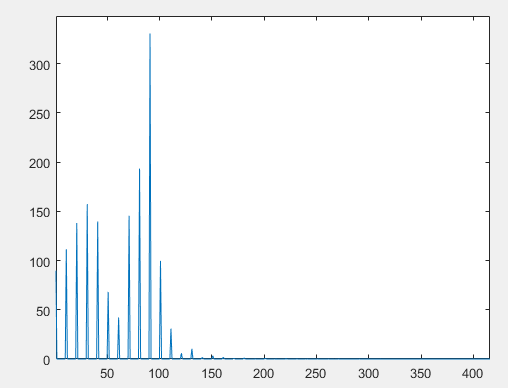
\includegraphics[scale = 0.75]{_045.PNG}\\[1.0 cm]
    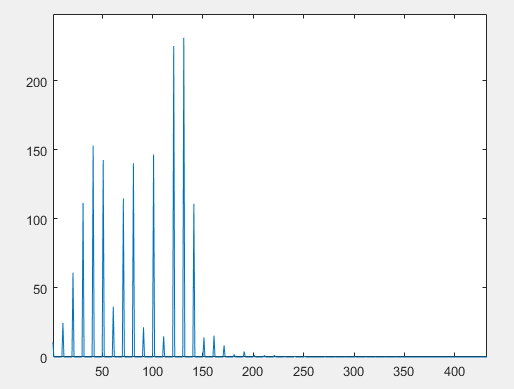
\includegraphics[scale = 0.75]{_065.PNG}\\[1.0 cm]
    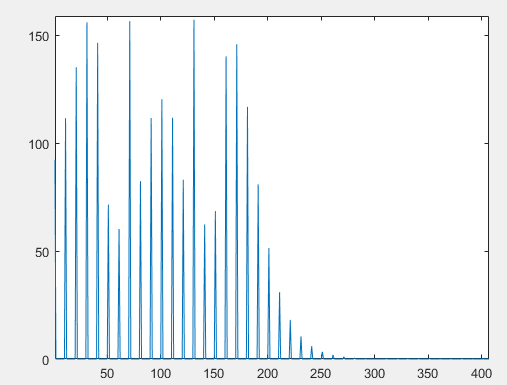
\includegraphics[scale = 0.75]{_095.PNG}\\[1.0 cm]
    
\end{center}
\end{flushleft}
\begin{table}[!h]
\centering
\begin{tabular}{c|c}
$\tau_{actual}$ & $\tau_{simulated}$ \\\hline
0.002 & 0.002 $\pm$ 0.0005 \\
0.015 & 0.015 $\pm$ 0.0005 \\
0.045 & 0.045 $\pm$ 0.0005 \\
0.065 & 0.065 $\pm$ 0.0005 \\
0.095 & \textit{Cannot evaluate due to multiple spikes  }
\end{tabular}
\caption{\label{Table 2: } Values of $\tau$ measured from simulation compared to actual values}
\end{table}
\textbf{Inferences:}\\
It can be seen that our method is effective as it just involved evaluating the value of freq at the spike.
Thus when we are under the constraints, the results are correct with the error factor of 0.0005sec. \\
\textbf{\textit{NOTE: This is the scaled downed version, so in the actual situations, where the distance is even less so that the delay is very less as compared to those we have taken, so error will even decrease further.}}
\subsubsection*{Effect of changing modulation factor}
Here we have kept $\tau$ to be equal to 0.02 and are analyzing the spectrum by changing $k_f$. The values of modulation factor are 20 and 100 respectively.
\begin{center}
     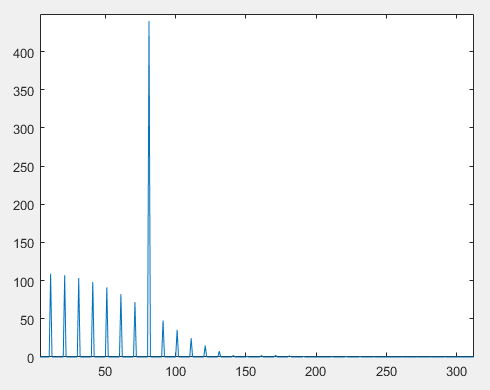
\includegraphics[scale = 0.75]{20.PNG}\\[1.0 cm]
     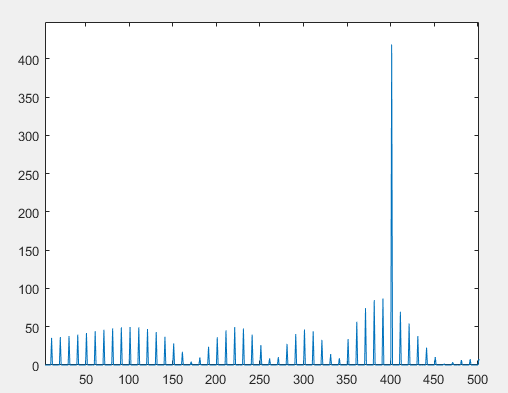
\includegraphics[scale = 0.75]{100.PNG}\\[1.0 cm]
\end{center}
\textbf{Inferences:} \\
It can be seen that increasing the value of modulation index decreases the relative magnitude of side lobes, but introduces more side lobes because the flat frequency is increasing. Hence the contribution of other frequency also increases. Increasing $k_f$ means increase in power transmitted, so which in turn is not good as far as practicality is concerned.
\section*{Multiple Object Detection}
\begin{flushleft}
Our technique works to Multiple objects as well. It is similar to the single object detection, However we will have multiple cosines in after mixer and LPF output. This causes multiple peaks at their corresponding frequencies.\\
\[r(t) = cos(2\pi f_c\tau_1+2\pi k_f \int_{t- \tau_1}^{t} m(x) dx )+ cos(2\pi f_c\tau_2+2\pi k_f \int_{t- \tau_2}^{t} m(x) dx )\]
Following is the spectrum obtained for this signal for different values of $\tau_1$ and $\tau_2$. \textbf{\textit{Note that for the successful detection from our method, the maximum of the 2 delays has to be less than $\frac{1}{2f_o}$}}.
\begin{center}
    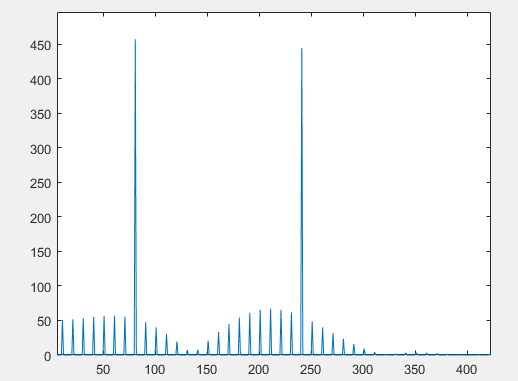
\includegraphics[scale = 0.60]{a.PNG}\\[1.0 cm]
    $\tau_1= 0.005$ and $\tau_2=0.015$\\
    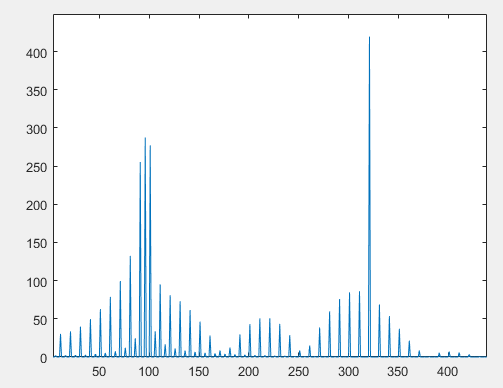
\includegraphics[scale = 0.6]{b.PNG}\\[1.0 cm]
    $\tau_1= 0.006$ and $\tau_2=0.020$\\
    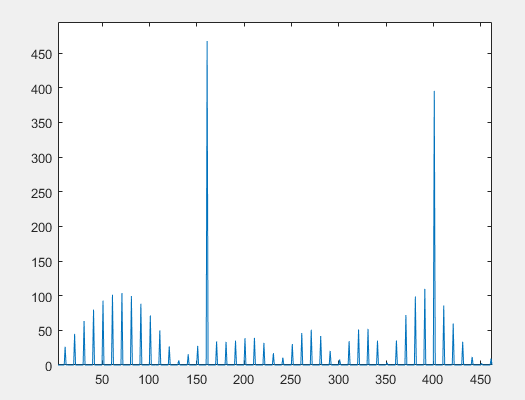
\includegraphics[scale = 0.75]{c.PNG}\\[1.0 cm]
    $\tau_1= 0.01$ and $\tau_2=0.025$\\
\end{center}
\textbf{Inferences}:
It can be seen that in this case we had more side lobes as compared to single object detection. Also the number of interference has increased in freq domain causing it difficult to see in freq domain clearly. \textit{\textbf{Thus it can be seen that for a clear detection we must have 2 delays little apart(otherwise we will have distortion due to interference) and the greater delay should be less than $\frac{1}{2f_o}$.}}
\end{flushleft}
\section*{Effect of Noise on the spectrum}
Adding an AWGN noise with the input causes non zero spectrum at every point. For the SNR 10 following is the filtered output. In the actual process, we need to pass the mixer output with the low pass filter. Since the model of noise is AWGN with 0 mean and variance $\sigma^2$, after passing through the filter, the noise would become 0 mean and variance $\sigma^2B_T $, where $B_T$ is the bandwidth determined by the Carson's Rule.
\begin{center}
     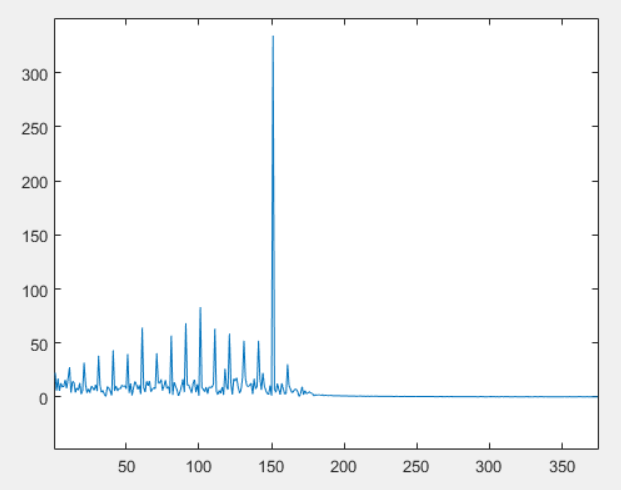
\includegraphics[scale = 0.75]{n1.PNG}\\[1.0 cm]
     $\tau= 0.015$ and $SNR=10$\\
     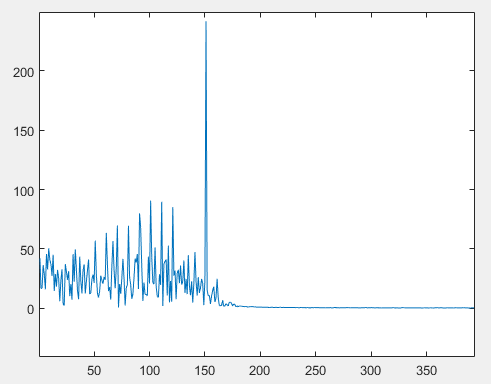
\includegraphics[scale = 0.75]{n+.PNG}\\[1.0 cm]
     $\tau= 0.015$ and $SNR=1$\\
     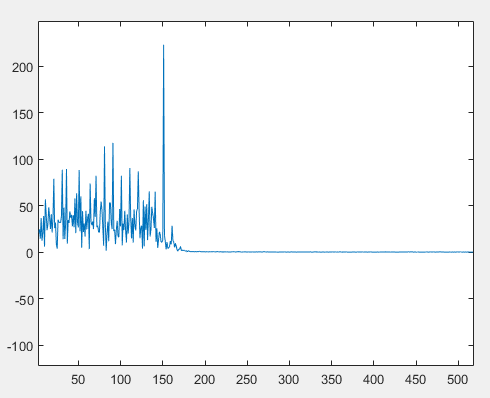
\includegraphics[scale = 0.75]{n++.PNG}\\[1.0 cm]
     $\tau= 0.015$ and $SNR=0.01$\\
     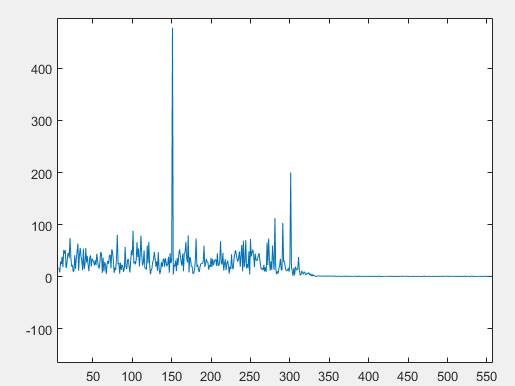
\includegraphics[scale = 0.75]{mulnoise.PNG}\\[1.0 cm]
     $\tau_1= 0.015$, $\tau_2= 0.03$ and $SNR=0.1$\\
\end{center}
\textbf{Inferences:}
Thus it can be seen that as the SNR decreases the noise effect increases and causing much more disturbance. However, the method is still valid as long as $\tau \leq \frac{1}{2f_o}$.\textit{ \textbf{However in the case of Multi-Object detection, in low SNR region we cannot say that the another spike so received whether is for noise or for signal. Thus we loose accuracy at low SNR regions in multi-object detection.}}
\section*{Results and Discussions}

\begin{itemize}
    \item Although the implementation of zero counting is easier as compared to the hardware implementation of FFT, we saw that FFT method surpasses the time- domain analysis even in the case when we have noise. In case of noise, the time domain analysis will fail badly. So we saw a trade-off in precision and cost optimization.
    \item The practical limit on $\tau$ is set by the frequency of the modulating signal. The maximum distance of detection is $\frac{c}{4f_o}$, as the max delay for good detection was $\frac{1}{2f_o}$.
    \item The noise after filtering will become a Gaussian random variable with 0 mean and variance of $\sigma^2$W where W is the bandwidth of LPF. Thus time domain method will have a high probability of error and we need to determine the threshold values practically for best prediction. 
    \item Due to computation constraints, we plotted things for up scaled values of delays. Similar results would come at the downscaled values of delays. Our analysis show the variation in spectrum by varying delays, parameters and adding noise to the system.
\end{itemize}

\end{document}